CNNs are mostly designed for natural images which usually have three channels. To satisfy this constraint, we generated a three channel RGB image from three MR sequences as shown in Figure \ref{fig:Fig2}.
\begin{figure} [ht]
   \begin{center}
   \begin{tabular}{c}
   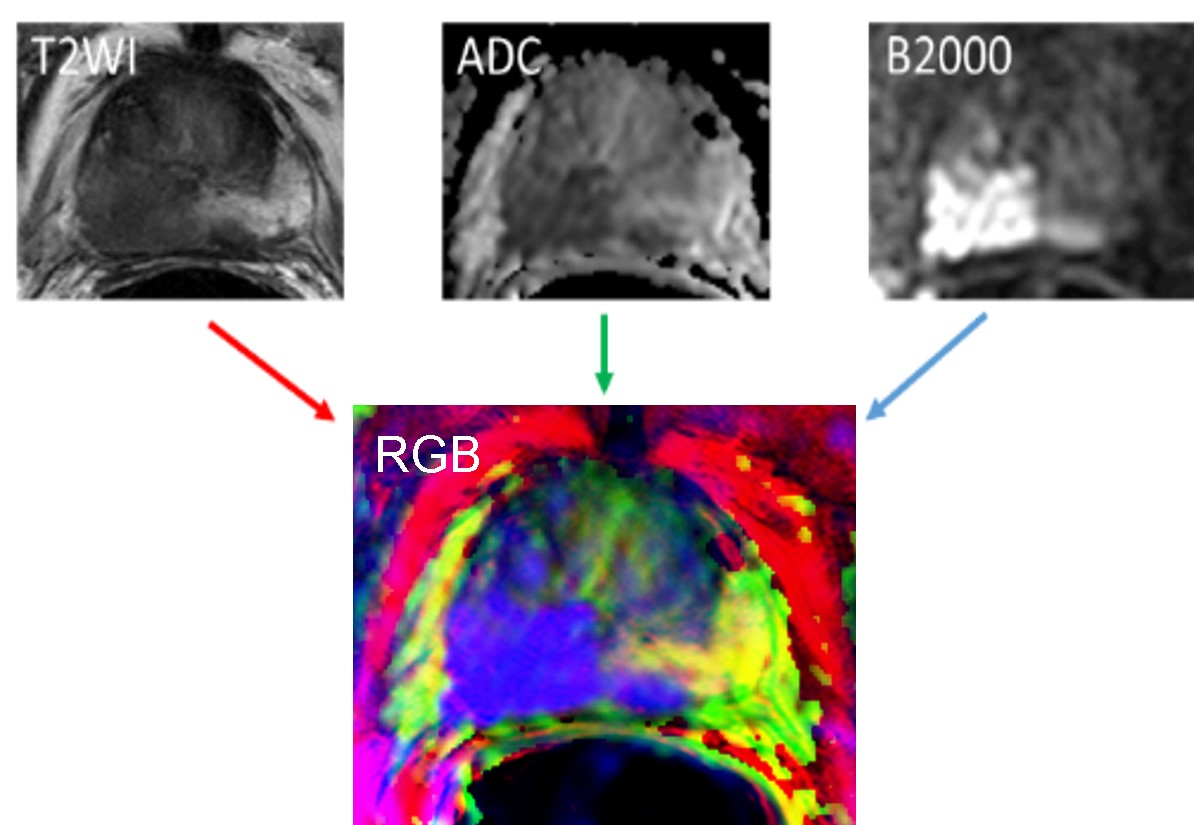
\includegraphics[height=5cm]{Figure2}
   \end{tabular}
   \end{center}
   \caption[Fig2]
   { \label{fig:Fig2} 
Generating a three channel RGB image from three mpMRIs.}
   \end{figure} 
Most publicly available CNNs are further limited in the type of images they take as input into their architecture. Usually, the input must be an 8 bit image with intensity values between 0 and 255; however, medical images such as the mpMRIs that we used are 12-16 bit with intensity values extending to upwards of 4000. We performed histogram equalization for all images to minimize information loss during compression. The three image sequences were processed separately before combining them into a single RGB image as in Figure \ref{fig:Fig2}. Figure \ref{fig:Fig3} shows the effects of using a histogram equalizing algorithm. The output from this algorithm has more contrast as compared to an output that uses linear compression according to Equation~(\ref{eq:eq1}).
\begin{equation}
\label{eq:eq1}
I^{\prime} = \frac{255\cdot I}{\max{X}}\,,
\end{equation}
where $I$ is the original mpMRI intensity value for a single pixel, $I'$ is the compressed intensity value, and $X$ is the input image.
\begin{figure} [tbh!]
   \begin{center}
   \begin{tabular}{c}
   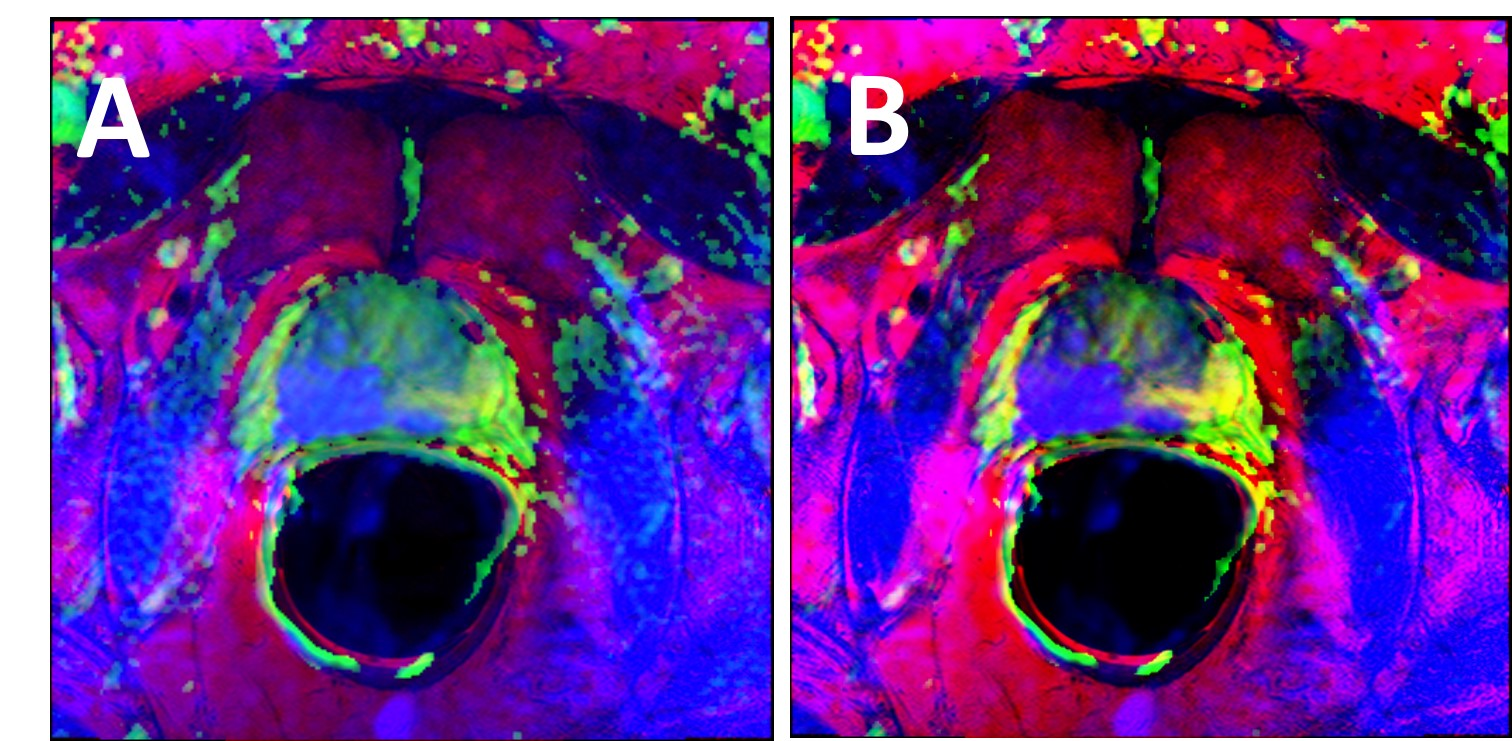
\includegraphics[height=5cm]{Figure3}
   \end{tabular}
   \end{center}
   \caption[Fig3]
   { \label{fig:Fig3} 
\textbf{(A)} is compressed in a linear fashion and without the use of histogram equalization. 
\textbf{(B)} Uses histogram equalization and shows more contrast within the image}
   \end{figure}
Lastly, prostate-masks were used to crop the images enabling the learning algorithm to ignore regions outside the prostate. 


